%! Author = ASUS
%! Date = 3/27/2023

% Preamble
\documentclass[11pt]{article}

% Packages
\usepackage{amsmath}
\usepackage{lipsum}
\usepackage{wasysym}
\usepackage{subcaption}
\usepackage{graphicx}
\usepackage{float}
\usepackage{listings}
\usepackage{xcolor}
\usepackage{pgfplots}
\lstset{basicstyle=\ttfamily,
  showstringspaces=false,
  commentstyle=\color{red},
  keywordstyle=\color{blue}
}

\graphicspath{{./images}}

% Document
\begin{document}
    \section{COLMAP}
    \paragraph{COLMAP} is an open source software, implemented by ~\cite{schoenberger2016sfm} and ~\cite{schoenberger2016mvs},
    that provides 3D reconstruction based on 2D images. The software comes with graphical user interface and
    command-line options that let it to be integrated easily with any other projects. It, also, has a great software
    architecture that makes it a powerful and flexible tool with a wide range of options for customization. COLMAP has
    shown a superb performance in compare to other SfM softwares, and it is being used widely in industry for
    core applications such as 3D modeling and robotics.

    \paragraph{Spare and Dense Reconstructions} are both implemented in COLMAP. Sparse reconstruction results in
    the 3D point cloud of only the detected features, while dense reconstruction refers to the point cloud of all
    pixels in the input images. Dense reconstrution is achievable after obtaining sparse reconstruction with camera
    poses. By default, It runs PatchMatch algorithm \cite{journals/tog/BarnesSFG09}, and it is a high time-consuming task.
    Through our project, sparse reconstruction is only considered.

    \paragraph{Customization} is the most important feature in this project. Each step of SfM pipline can be executed
    separately. Hence, any other algorithm can be repalced by its defaults. And, any extra steps, like refinements,
    can be added to the pipeline. Moreover, every single default step has a range of options to change, such as
    the maximum number of features and matches, thresholds, different camera settings with fixed camera parameters, etc.
    Here is sample bash code that shows an overview of our customization applied to the feature detection step:

    \begin{lstlisting}[language=bash,caption={colmapsparse.sh},label={lst:lstlisting2}]
        #!/bin/bash

        colmap feature_extractor \
           --database_path $DATASET_PATH/database.db \
           --image_path $DATASET_PATH/images \
           --SiftExtraction.max_image_size 10000 \
           --SiftExtraction.max_num_features 20000 \
           --SiftExtraction.estimate_affine_shape 1 \
           --ImageReader.single_camera 1 \
           --ImageReader.camera_model FULL_OPENCV \
           --ImageReader.camera_params $CALIB_PARAMS_YAML
    \end{lstlisting}

    \paragraph{In our experiment}, COLMAP is used for 3D reconstruction with different settings. Pixel-Perfect
    refinement codes are placed between COLMAP pipeline after initial keypoints detection. Also, we will see that
    by manipulating COLMAP options, it can be used in vSLAM too.

    \newpage

    \section{Data acquisition}
    \paragraph{GoPro cameras} are small, portable, and captures high quality videos in high frame rates. They also, provide
    a programming api that makes it super easy to develop applications based the cameras' output. Hence, they
    are popular in computer vision and robotics researches. In our experiment, the GoPro 9 camera was fixed on
    a bike, and several videos were taken from the city of Padua, while riding through the streets.

    \paragraph{Our dataset} is created from the two videos captured by the following camera settings:

    \begin{enumerate}
        \item
        \begin{itemize}
            \item 10 minutes, 1080p, 60 frames/sec, Undistorted
            \item SfM input images are every 10 frames from the video, means 6 images per second
        \end{itemize}
        \item
        \begin{itemize}
            \item 25 minutes, 2.7k, 60f, wide and distorted
            \item SfM input images are every 15 frames, 2704×1538 dimensions
        \end{itemize}
    \end{enumerate}

    \paragraph{Extra data:} GoPro cameras come with additional information for the captured videos, such as GPS, IMU.
    https://github.com/gopro/gpmf-parser is the application used to extract these data from video files. Sample GPS
    data of the first 5 seconds:

    \begin{lstlisting}[language=bash,caption={gpmf-parser output},label={lst:lstlisting}]
        VIDEO FRAMERATE:
        59.940 with 31860 frames
        PAYLOAD TIME:
          0.000 to 1.001 seconds
        SCALED DATA:
          GPS5 45.406deg, 11.877deg, 19.839m, 2.418m/s, 2.450m/s,
          GPS5 45.406deg, 11.877deg, 19.831m, 2.432m/s, 2.420m/s,
          GPS5 45.406deg, 11.877deg, 19.816m, 2.489m/s, 2.430m/s,
          GPS5 45.406deg, 11.877deg, 19.811m, 2.501m/s, 2.490m/s,
          GPS5 45.406deg, 11.877deg, 19.807m, 2.501m/s, 2.500m/s,
          GPS5 45.406deg, 11.877deg, 19.821m, 2.495m/s, 2.500m/s,
          GPS5 45.406deg, 11.877deg, 19.828m, 2.503m/s, 2.500m/s,
          GPS5 45.406deg, 11.877deg, 19.830m, 2.505m/s, 2.500m/s,
          GPS5 45.406deg, 11.877deg, 19.825m, 2.520m/s, 2.510m/s,
          GPS5 45.406deg, 11.877deg, 19.819m, 2.493m/s, 2.520m/s,
          GPS5 45.406deg, 11.877deg, 19.822m, 2.472m/s, 2.490m/s,
          GPS5 45.406deg, 11.877deg, 19.820m, 2.471m/s, 2.470m/s,
          GPS5 45.406deg, 11.877deg, 19.822m, 2.494m/s, 2.470m/s,
          GPS5 45.406deg, 11.877deg, 19.790m, 2.448m/s, 2.490m/s,
          GPS5 45.406deg, 11.877deg, 19.775m, 2.444m/s, 2.450m/s,
          GPS5 45.406deg, 11.877deg, 19.775m, 2.434m/s, 2.440m/s,
          GPS5 45.406deg, 11.877deg, 19.759m, 2.404m/s, 2.430m/s,
          GPS5 45.406deg, 11.877deg, 19.763m, 2.412m/s, 2.400m/s,
        PAYLOAD TIME:
          1.001 to 2.002 seconds
        SCALED DATA:
          GPS5 45.406deg, 11.877deg, 19.763m, 2.411m/s, 2.410m/s,
          GPS5 45.406deg, 11.877deg, 19.751m, 2.412m/s, 2.410m/s,
          GPS5 45.406deg, 11.877deg, 19.767m, 2.443m/s, 2.410m/s,
          GPS5 45.406deg, 11.877deg, 19.749m, 2.455m/s, 2.440m/s,
          GPS5 45.406deg, 11.877deg, 19.757m, 2.455m/s, 2.460m/s,
          GPS5 45.406deg, 11.877deg, 19.780m, 2.436m/s, 2.460m/s,
          GPS5 45.406deg, 11.877deg, 19.796m, 2.448m/s, 2.440m/s,
          GPS5 45.406deg, 11.877deg, 19.770m, 2.426m/s, 2.450m/s,
          GPS5 45.406deg, 11.877deg, 19.788m, 2.441m/s, 2.430m/s,
          GPS5 45.406deg, 11.877deg, 19.794m, 2.462m/s, 2.440m/s,
          GPS5 45.406deg, 11.877deg, 19.815m, 2.480m/s, 2.460m/s,
          GPS5 45.406deg, 11.877deg, 19.837m, 2.504m/s, 2.480m/s,
          GPS5 45.406deg, 11.877deg, 19.859m, 2.523m/s, 2.500m/s,
          GPS5 45.406deg, 11.877deg, 19.882m, 2.473m/s, 2.520m/s,
          GPS5 45.406deg, 11.877deg, 19.898m, 2.482m/s, 2.470m/s,
          GPS5 45.406deg, 11.877deg, 19.899m, 2.484m/s, 2.480m/s,
          GPS5 45.406deg, 11.877deg, 19.905m, 2.496m/s, 2.480m/s,
          GPS5 45.406deg, 11.877deg, 19.913m, 2.490m/s, 2.500m/s,
          GPS5 45.406deg, 11.877deg, 19.915m, 2.517m/s, 2.490m/s,
        PAYLOAD TIME:
          2.002 to 3.003 seconds
    \end{lstlisting}

    We will see initial pose for cameras can boost SfM pipeline enormously. However, GPS data from GoPro cameras
    are not usable in this process.
    GPS sampling rate is 18 per second. It means there are 18 position data in one second. However, after reviewing
    all GPS data for a long video, we realized that the coordinates are updated every 2 or 3 seconds which is not ideal.
    In SFM, the algorithm finds the coordinates of the camera for each frame. If we want to use GPS data as an initial
    value in SFM, 40 to 60 frames might have the same initial coordinates which doesn't help the algorithm.
    Moreover, GPS data from GPMF metadata has an accuracy of three-tenth of a decimal. We checked this error in
    Google Maps, and the error could be 10 meters. While, SFM has an error of less than a centimeter.

    \paragraph{Reconstruction}: The extracted frames are then grouped into batches and fed into COLMAP SfM pipeline.

    The first dataset is from the undistorted video. For the ease of recalling, we will call this dataset
    "The First dataset". The first dataset is made from 120 frames with resolution of 1920*1088, and size of ~3MB
    for each image. The figure \ref{fig:1ply} is the sparse reconstruction obtained by COLMAP:

    \begin{figure}
    \caption{The First Dataset: Sparse and Dense Point Cloud}
    \centering
    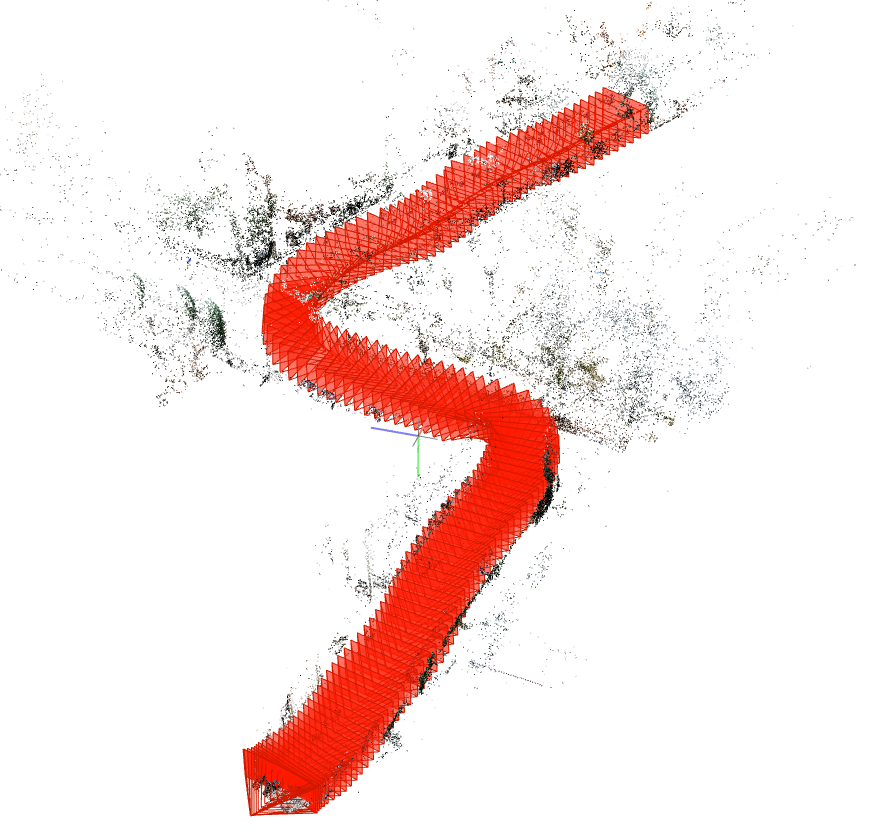
\includegraphics[width=\textwidth,height=\textheight,keepaspectratio]{images/1.ply.sparse.png}
    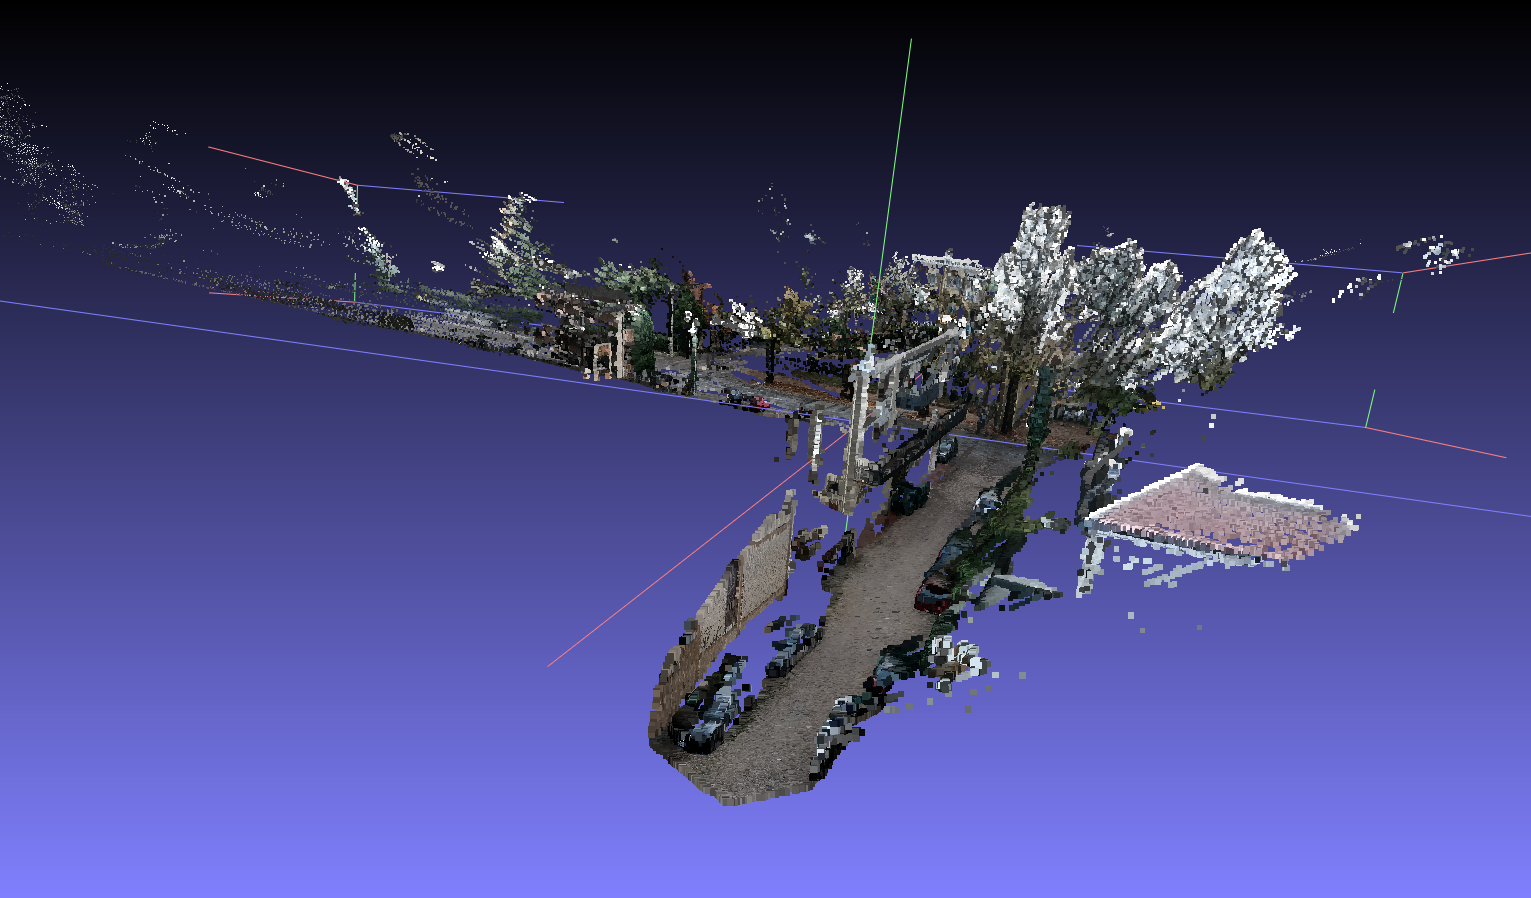
\includegraphics[width=\textwidth,height=\textheight,keepaspectratio]{images/1.ply.dense.1.png}
    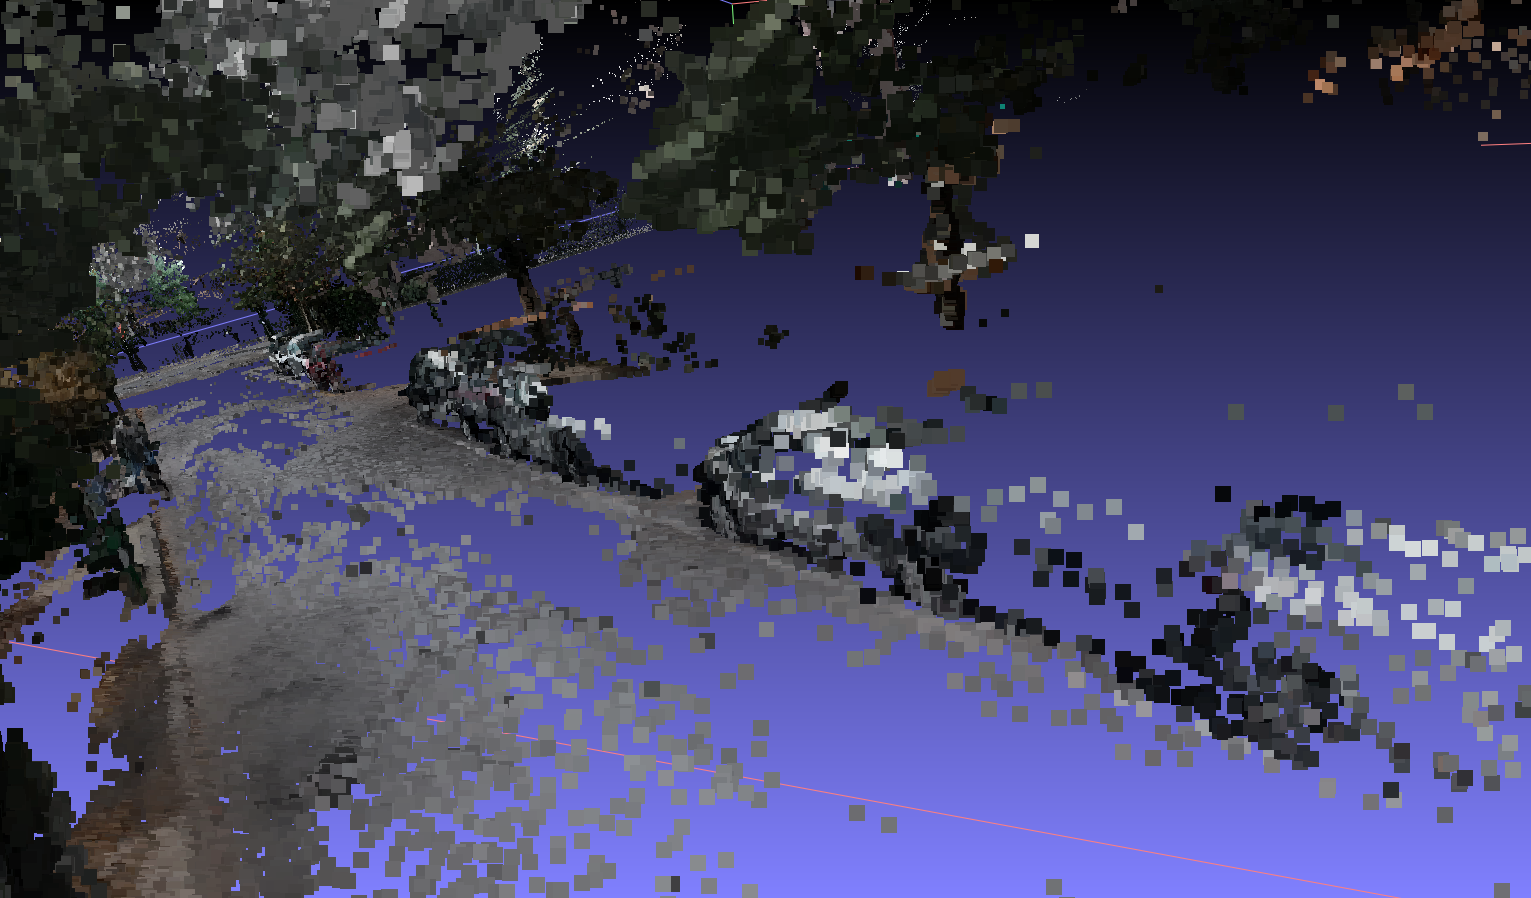
\includegraphics[width=\textwidth,height=\textheight,keepaspectratio]{images/1.ply.dense.2.png}
    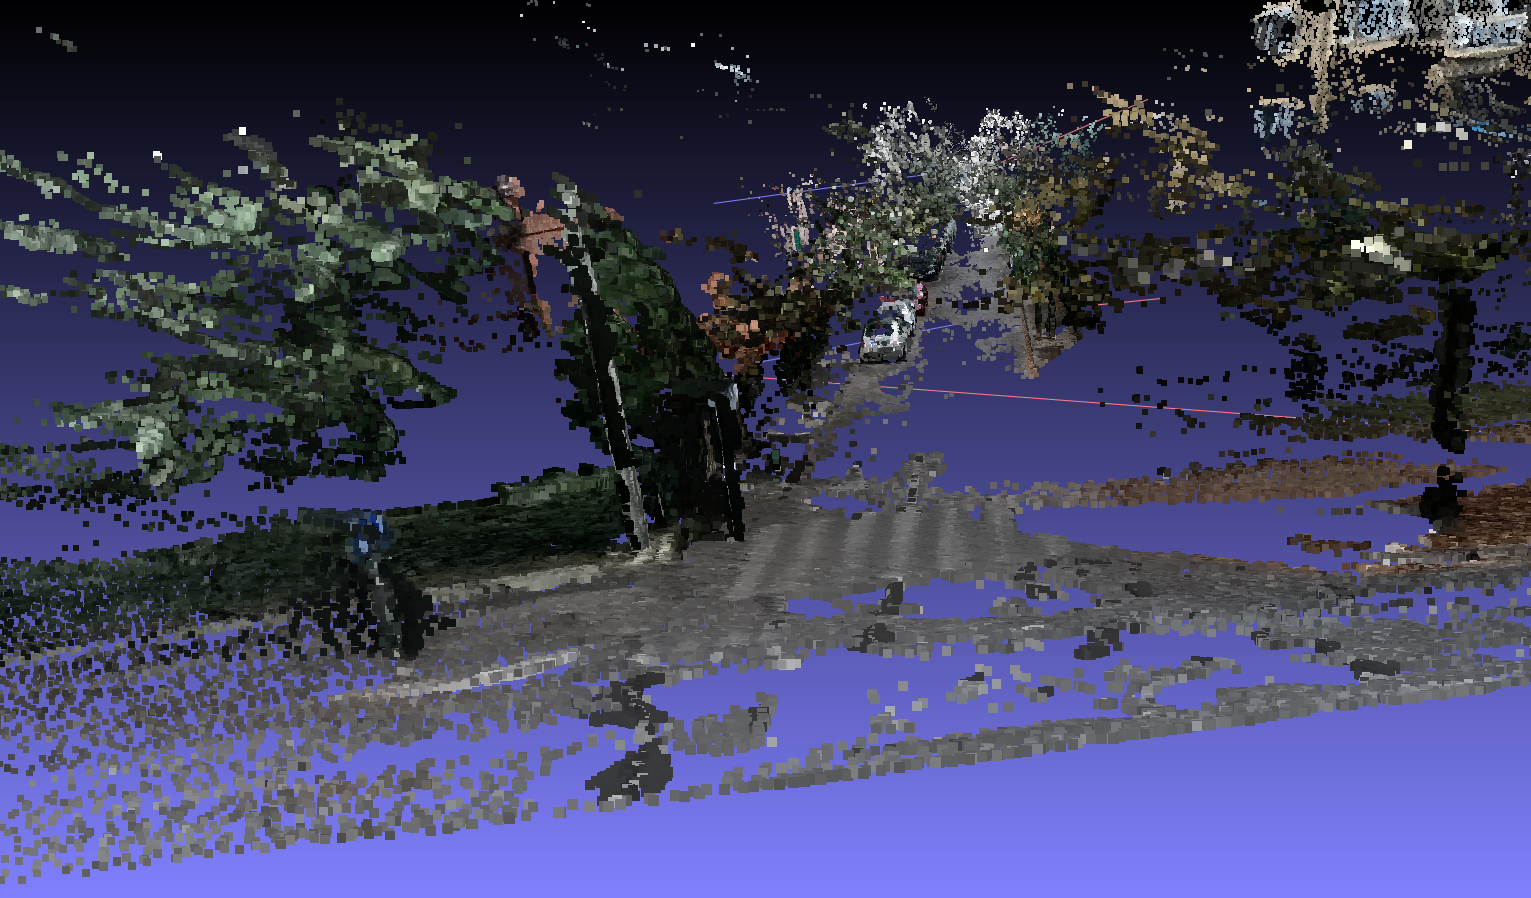
\includegraphics[width=\textwidth,height=\textheight,keepaspectratio]{images/1.ply.dense.3.png}
    \label{fig:1ply}
    \end{figure}

    The Second Dataset is from 2.7k video, and contains 175 distorted images. The final point cloud includes
    100k points. The reconstrution is shown in the figure \ref{fig:2ply}

    \begin{figure}
    \caption{The Second Dataset: Sparse and Dense Point Cloud}
    \centering
    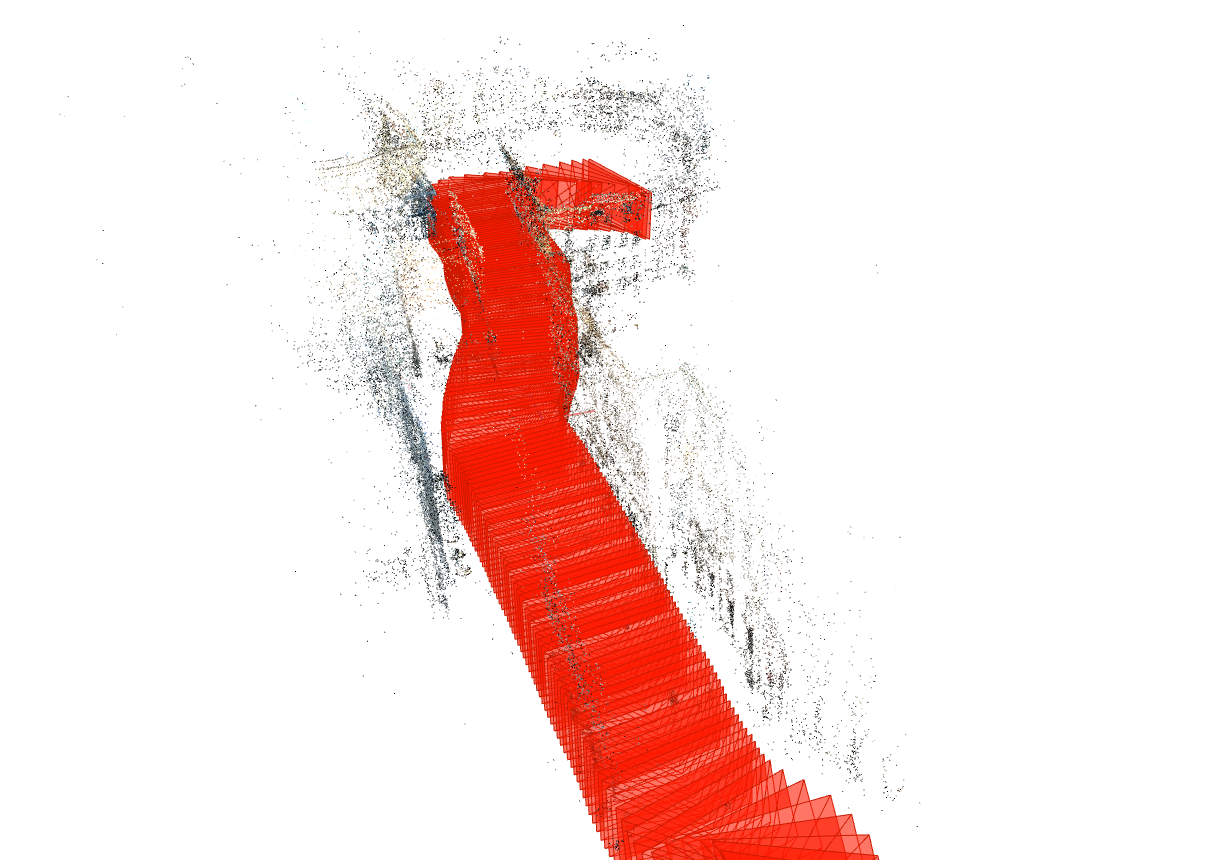
\includegraphics[width=\textwidth,height=\textheight,keepaspectratio]{images/2.ply.sparse.png}
    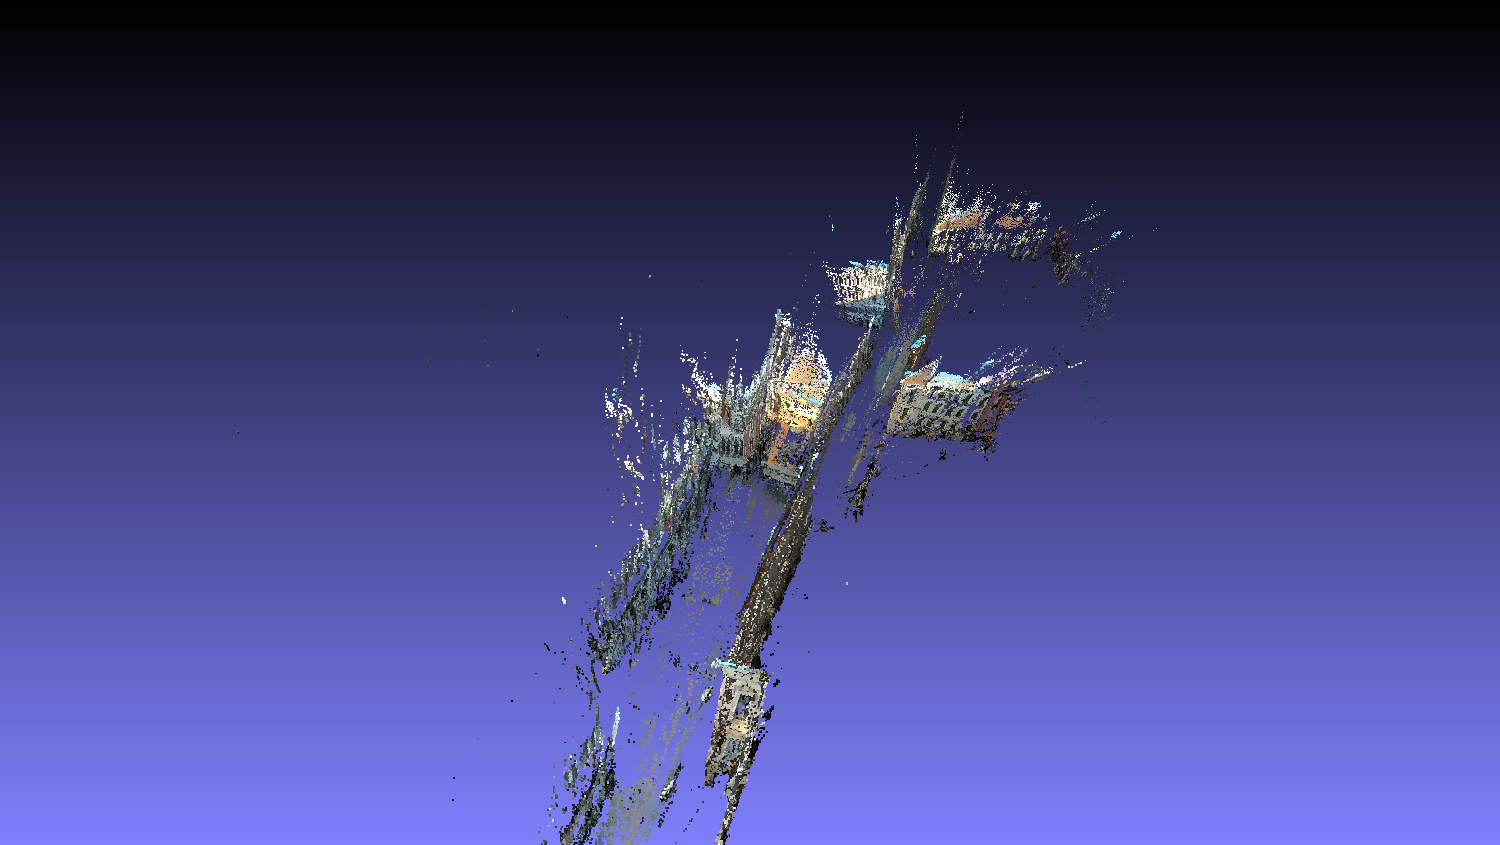
\includegraphics[width=\textwidth,height=\textheight,keepaspectratio]{images/2.ply.dense.1.png}
    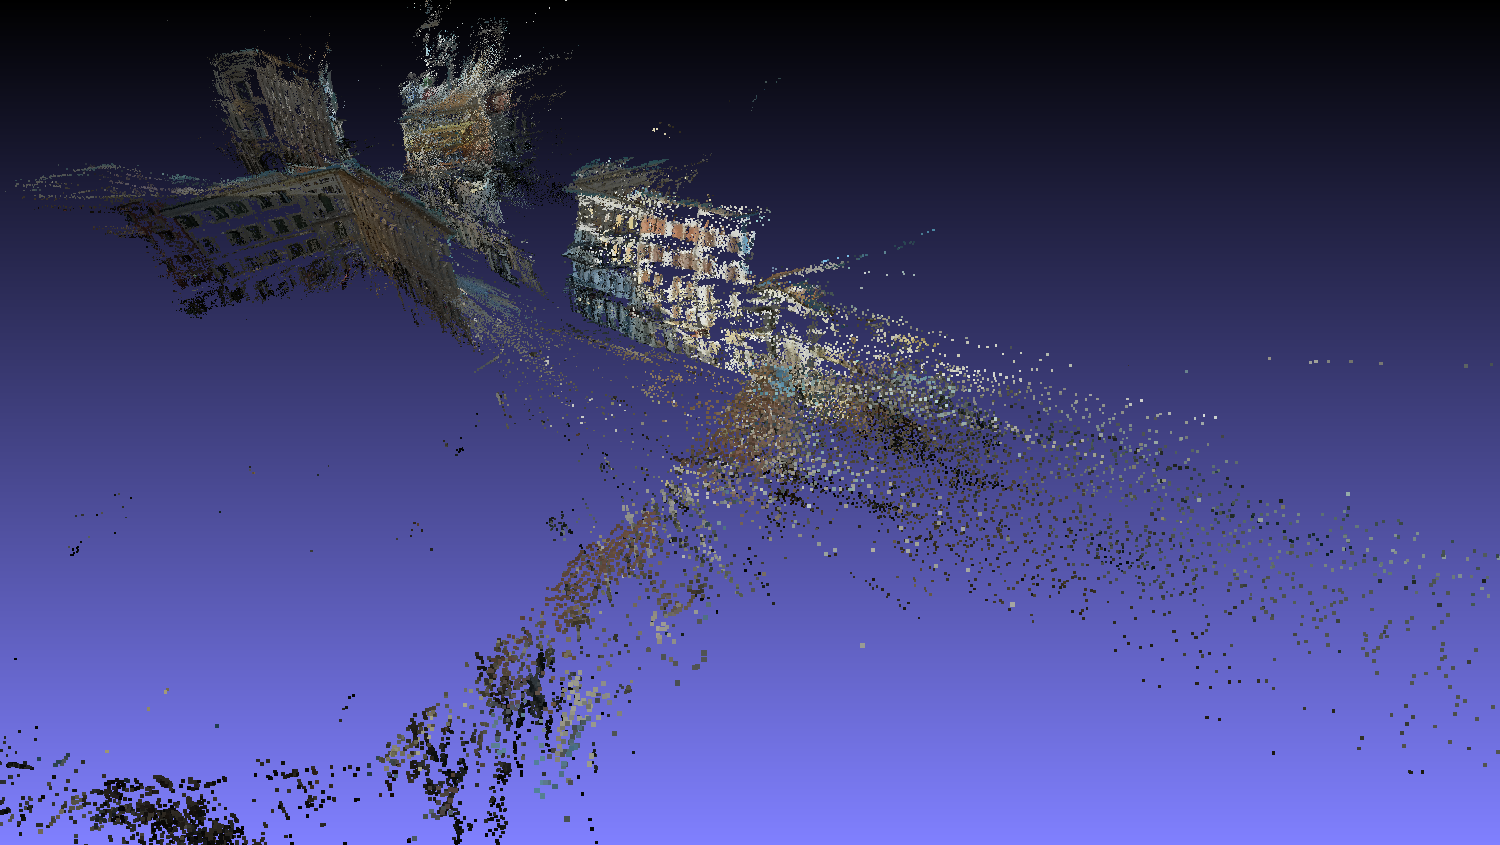
\includegraphics[width=\textwidth,height=\textheight,keepaspectratio]{images/2.ply.dense.2.png}
    \label{fig:2ply}
    \end{figure}

    \section{Refinement}
    ~\cite{lindenberger2021pixsfm} is described in detail in the previous chapter. Here, we apply this approach to
    refine our point clouds.

    \section{Compare the results with City point cloud}
    
    \section{Calibration and its imapct}

    \section{Real-Time Structure from Motion}

    \section{Dataset}
    1) Aerial Point Cloud: An extensive collection of 3D points is obtained from the city of Padova
    using an airplane. The covered region spans 1600m by 1000m, and the average nearest neighbor distance
    of points is 0.63m. The dataset contains a total of 3,583,803 points.
    2) Ground Point Clouds: 10 dense point clouds are created using the Structure from Motion techniques.
    These datasets are further refined using Pixel-Perfect algorithm. Each dataset comprises an average of
    60 frames extracted from a 30-second undistorted video. The video was recorded at a frame rate of 60 fps,
    resulting in the generation of point clouds at a rate of 2 pictures per second. The resolution of each image
    is 1920*1088 pixels, and the distance covered in each dataset ranges from 80 to 120 meters.

    #TODO: add images

    \section{Point Cloud Registration}
    The objective is to align the ground point cloud with the aerial point cloud. Initially, we attempted
    to register the point cloud using traditional global and local algorithms like FPFH feature matching,
    RANSAC, and ICP. However, due to significant differences in the nature of the datasets, the results were
    too poor. The aerial point cloud primarily consists of street points and building roofs, as it is captured
    from above. While, the ground point cloud contains street points and building walls. Therefore, we need to
    find the common features and simplify the problem. The new pipeline could be described as follows:
    \begin{enumerate}
        \item It was observed that viewing both point clouds from above, aligned with the z-axis, provides
        valuable information. The first step is to align the point clouds with the z-axis. The aerial
        point cloud is already aligned. The ground point cloud is segmented into planes, and the plane
        with the highest point count is identified as the street plane, since it is the common plane among
        all streets and directions and so more points must be related to the ground plane. Then,
        the rotation matrix between the normal vector of the street plane and the (x=0, y=0, z=1) vector
        is computed and applied to the entire ground point cloud. This step roughly determines the rotation
        around x and y axes. Here is an elevation map from top point of view aligned with z axis:
        #TODO: images elevation maps

        \item From the top point of view, It is seen that the most discriminative feature among the datasets
        is the angles of streets and crossroads. So, the data of vertical walls in ground dataset and roofs
        in aerial dataset has no use. Therefore, both point clouds are sliced along the z-axis with a certain
        threshold, and the half related to the streets is remained. In the examples below, the similarity of
        both ground and aerial point clouds are
        #TODO: images

        \item Since the generated point clouds has the up-to-scale problem, it is needed to normalize the
        coordinate values across all datasets. This step does not scale the ground point clouds to the actual size
        in aerial point cloud. However, it ensures that the average minimum distance between the points is 1px.
        Each point cloud is scaled by the factor of 1 divided by the average of the minimum distance to the nearest point.

        \item A 2D binary map is generated for each point cloud considering only x and y coordinates of each 3D point.
        The dimensions of the map are determined by calculating the difference between the maximum and minimum x and y
        coordinates of all points and dividing it by a predefined resolution value. Each cell in the map is assigned
        a value of 1 if at least one point's x and y coordinates fall within that cell, indicating the presence of
        points in that area. Conversely, if there are no points corresponding to the respective x and y coordinates,
        the cell is marked as 0. In the binary grid map for Ground Point Cloud, considering that each point cloud is
        generated from a sequence of video frames, the camera pose of the middle frame is regarded as the ground truth
        center position for the entire dataset. To evaluate the registration method's robustness and generalization,
        3 aerial point clouds are considered for each ground dataset. These aerial point clouds share the same center
        as the aforementioned ground point cloud, but they differ in distance from the center. They are categorized
        as "easy," "medium," and "hard" with distances of 100, 150, and 200 meters from each direction, respectively.
        The binary grid map is generated for these aerial point clouds using the same logic as the binary grid map
        created for the ground point clouds.

        \item To localize the ground grid map within the aerial grid maps, various methods were explored, including
        2D feature matching, crossroad detection based on point counting, and training convolutional neural networks,
        etc. Among these approaches, template matching has the best results. The template matching process involves
        comparing a small template image, which represents the desired pattern (in this case, the ground grid map),
        with different regions of the target image (the aerial grid map). The objective is to identify the best match
        or similarity between the template and the target image. This is achieved by moving a window across the target
        image and comparing the template with each window. We also extended the algorithm to also includes different
        scaling and rotation parameters. The template is rotated upto 360 degrees with an interval of 10 degrees and
        scaled from 10\% to 200\% of its initial size, increasing 10 percent for each attempt.

    \end{enumerate}

    The whole pipeline can be summarized as follows:
    \begin{enumerate}
        \item Take the video of the streets, and extract the frames
        \item Run sparse SfM algorithm
        \item Refine the sparse point cloud and camera poses using Pixel Perfect algorithm
        \item Generate a dense point cloud from the refined data
        \item Align the point cloud along the z-axis.
        \item Scale and Slice the ground point cloud, and keep the points with z coordinate less than a threshold,
        in our case, the threshold is 20\% of the minimum z-coordinate
        \item Generate the binary grid map
        \item Slice Aerial point cloud along the z-axis with certain threshold, in our case, the threshold is 20\%
        of the minimum of z coordinate of all points
        \item Generate Binary grid map for Aerial point cloud
        \item Run Template Matching algorithm to localize the ground grid map inside the aerial grind map
    \end{enumerate}

    \section{Metrics}
    In our matching problem, there are four key parameters for evaluation:
    \begin{itemize}
        \item the 2D coordinates (x, y) of the detected pose of the center,
        \item the scale
        \item the rotation
    \end{itemize}
    of the ground binary grid map within the source binary grid map.

    The results of the global registration are binary in nature, meaning that whether the template point cloud
    is successfully found in the source or not. Hence, the first metric used is the Average Success Rate.
    \paragraph{Average Success Rate:} For each ground binary map and its corresponding aerial binary map, if the difference
    between the four key parameters and their ground truth values is less than a certain threshold, it is considered
    a successful match. In our experiment, the euclidean distance between the center of ground binary map and the ground
    truth, i.e. which is the center of each aerial binary grid map, should not be more than 25 meters. An acceptable
    scale factor is between 80\% to 130\% of the ground truth. And, the rotation angle should non be more than 10
    degrees, otherwise, in most cases, the wrong street is detected.

    \section{Results}
    There are 10 ground datasets, and for each dataset, there are three aerial datasets categorized as easy, medium,
    and hard. The Figure X shows the average success rate, in percentage, for all ground datasets based on the
    difficulty level of their corresponding aerial datasets.

    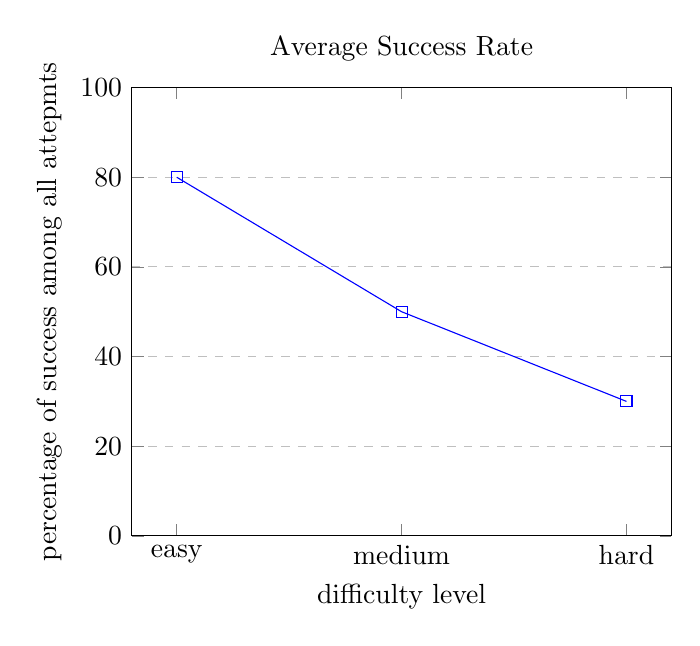
\begin{tikzpicture}
        \begin{axis}[
            title={Average Success Rate},
            xlabel={difficulty level},
            ylabel={percentage of success among all attepmts},
            ymin=0, ymax=100,
            xtick=data,
            xticklabels={easy, medium, hard,},
            ytick={0,20,40,60,80,100},
            legend pos=north west,
            ymajorgrids=true,
            grid style=dashed,
        ]

            \addplot[
                color=blue,
                mark=square,
                ]
                coordinates {
                (1,80)
                (2,50)
                (3,30)
                };
        \end{axis}
    \end{tikzpicture}

    Here are the final matches for the datasets. For each ground dataset, 3 images are provided illustrating the
    matches in easy, medium and hard aerial point clouds. The yellow pixels refer to the aerial point cloud(source)
    and green pixels are related to the ground point cloud(template). The axes of the graph are scaled in meters multiplied
    by a resolution value. This resolution is either 3.3 or 6.6 and is because of variations in the density of points
    and for a more accurate representation of the grid maps.

    For each ground dataset that has at least one successful result, a table of detailed errors of transformation
    in meters, i.e. distance between the center of source and template images, scale in percentage, and angle in
    degrees is provided.

    % 4_3_3
    \newpage
    \begin{figure}[p]
        \centering
        \begin{subfigure}{0.45\textwidth}
            \centering
            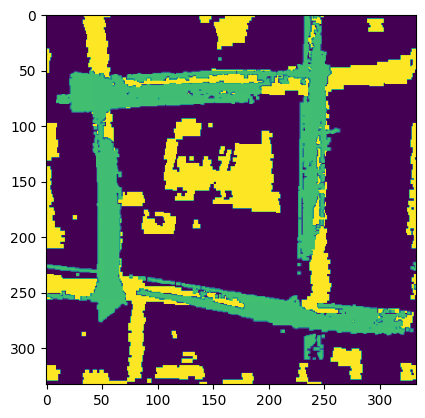
\includegraphics[width=\linewidth]{images/full/easy/4_3_3_easy}
            \caption{Easy: \textcolor{teal}{Success}}
            \label{fig:4_3_3_easy}
        \end{subfigure}
        \hfill
        \begin{subfigure}{0.45\textwidth}
            \centering
            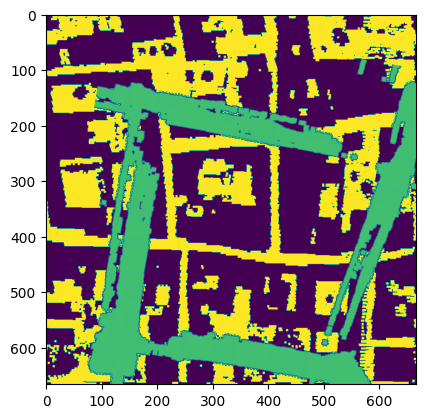
\includegraphics[width=\linewidth]{images/full/medium/4_3_3_medium}
            \caption{Medium: \textcolor{red}{Failed}}
            \label{fig:4_3_3_medium}
        \end{subfigure}

        \vspace{1em}

        \begin{subfigure}{0.45\textwidth}
            \centering
            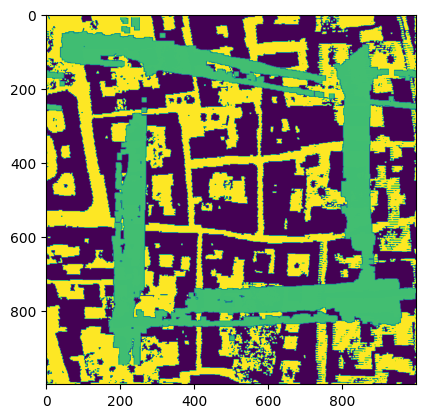
\includegraphics[width=\linewidth]{images/full/hard/4_3_3_hard}
            \caption{Hard: \textcolor{red}{Failed}}
            \label{fig:4_3_3_hard}
        \end{subfigure}
        \hfill

        \caption{Dataset 1}
        \label{fig:res_4_3_3}
    \end{figure}

    \begin{table}[p]
        \centering
        \begin{tabular}{|c|c|c|c|}
          \hline
          \textbf{Errors:} & \textbf{Transformation} & \textbf{Scale} & \textbf{Rotation} \\
          \hline
          \textbf{Easy} & 0.50m & +3.5\% & +2° \\
          \hline
          \textbf{Medium} & - & - & - \\
          \hline
          \textbf{Hard} & - & - & - \\
          \hline
        \end{tabular}
        \caption{Detailed errors of Dataset 1}
        \label{tab:simpletable}
    \end{table}

    % 4_1_3
    \newpage
    \begin{figure}[p]
        \centering
        \begin{subfigure}{0.45\textwidth}
            \centering
            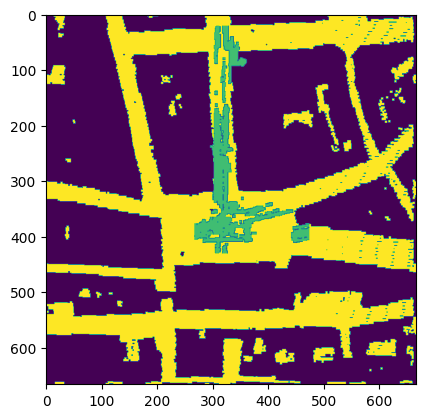
\includegraphics[width=\linewidth]{images/full/easy/4_1_3_easy}
            \caption{Easy: \textcolor{teal}{Success}}
            \label{fig:4_1_3_easy}
        \end{subfigure}
        \hfill
        \begin{subfigure}{0.45\textwidth}
            \centering
            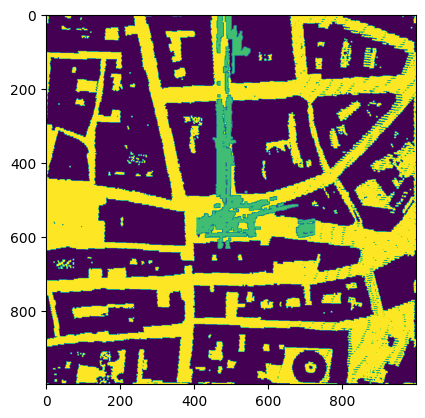
\includegraphics[width=\linewidth]{images/full/medium/4_1_3_medium}
            \caption{Medium: \textcolor{teal}{Success}}
            \label{fig:4_1_3_medium}
        \end{subfigure}

        \vspace{1em}

        \begin{subfigure}{0.45\textwidth}
            \centering
            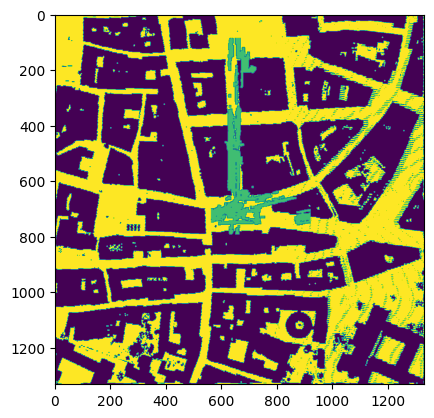
\includegraphics[width=\linewidth]{images/full/hard/4_1_3_hard}
            \caption{Hard: \textcolor{teal}{Success}}
            \label{fig:4_1_3_hard}
        \end{subfigure}
        \hfill

        \caption{Dataset 2}
        \label{fig:res_4_1_3}
    \end{figure}

    \begin{table}[p]
        \centering
        \begin{tabular}{|c|c|c|c|}
          \hline
          \textbf{Errors:} & \textbf{Transformation} & \textbf{Scale} & \textbf{Rotation} \\
          \hline
          \textbf{Easy}   & 3.16m & -8.7\%  & -3° \\
          \hline
          \textbf{Medium} & 6.66  & +7.14\% & -3° \\
          \hline
          \textbf{Hard}   & 26.6  & +16.6\% & -3° \\
          \hline
        \end{tabular}
        \caption{Detailed errors of Dataset 2}
        \label{tab:simpletable}
    \end{table}

    % 5_1_2
    \newpage
    \begin{figure}[p]
        \centering
        \begin{subfigure}{0.45\textwidth}
            \centering
            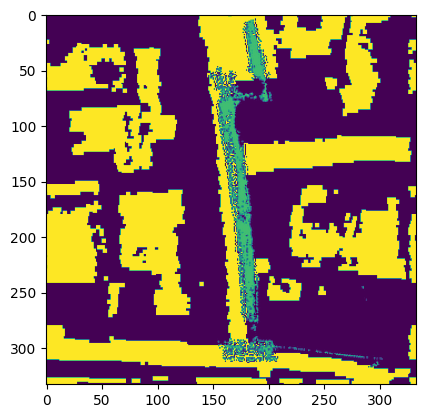
\includegraphics[width=\linewidth]{images/full/easy/5_1_2_easy}
            \caption{Easy: \textcolor{teal}{Success}}
            \label{fig:5_1_2_easy}
        \end{subfigure}
        \hfill
        \begin{subfigure}{0.45\textwidth}
            \centering
            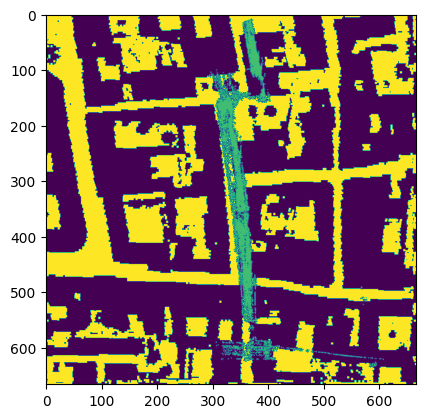
\includegraphics[width=\linewidth]{images/full/medium/5_1_2_medium}
            \caption{Medium: \textcolor{teal}{Success}}
            \label{fig:5_1_2_medium}
        \end{subfigure}

        \vspace{1em}

        \begin{subfigure}{0.45\textwidth}
            \centering
            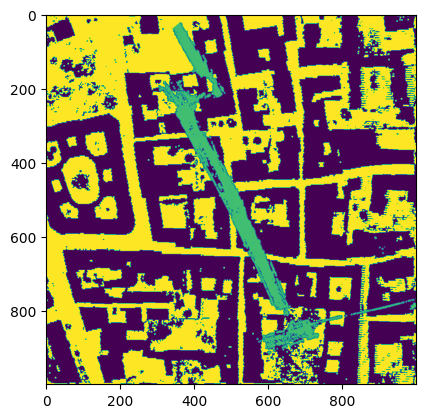
\includegraphics[width=\linewidth]{images/full/hard/5_1_2_hard}
            \caption{Hard: \textcolor{red}{Failed}}
            \label{fig:5_1_2_hard}
        \end{subfigure}
        \hfill

        \caption{Dataset 3}
        \label{fig:res_5_1_2}
    \end{figure}

    \begin{table}[p]
        \centering
        \begin{tabular}{|c|c|c|c|}
          \hline
          \textbf{Errors:} & \textbf{Transformation} & \textbf{Scale} & \textbf{Rotation} \\
          \hline
          \textbf{Easy}   & 1.6m & -4.4\%  & 1° \\
          \hline
          \textbf{Medium} & 4.83m  & +13.3\% & 1° \\
          \hline
          \textbf{Hard}   & -  & - & - \\
          \hline
        \end{tabular}
        \caption{Detailed errors of Dataset 3}
        \label{tab:simpletable}
    \end{table}

    % 4_0_1
    \newpage
    \begin{figure}[p]
        \centering
        \begin{subfigure}{0.45\textwidth}
            \centering
            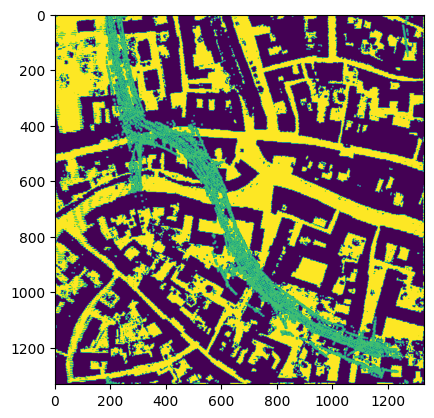
\includegraphics[width=\linewidth]{images/full/easy/4_0_1_easy}
            \caption{Easy: \textcolor{red}{Failed}}
            \label{fig:4_0_1_easy}
        \end{subfigure}
        \hfill
        \begin{subfigure}{0.45\textwidth}
            \centering
            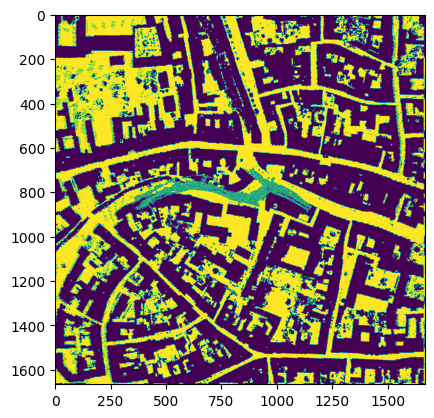
\includegraphics[width=\linewidth]{images/full/medium/4_0_1_medium}
            \caption{Medium: \textcolor{teal}{Success}}
            \label{fig:4_0_1_medium}
        \end{subfigure}

        \vspace{1em}

        \begin{subfigure}{0.45\textwidth}
            \centering
            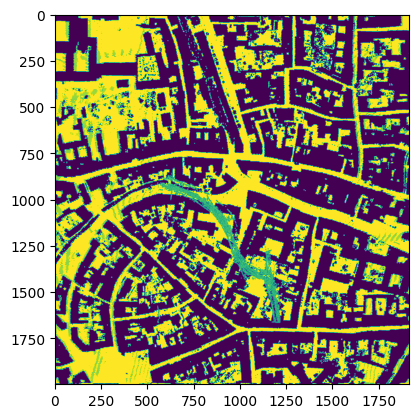
\includegraphics[width=\linewidth]{images/full/hard/4_0_1_hard}
            \caption{Hard: \textcolor{red}{Failed}}
            \label{fig:4_0_1_hard}
        \end{subfigure}
        \hfill

        \caption{Dataset 4}
        \label{fig:res_4_0_1}
    \end{figure}

    \begin{table}[p]
        \centering
        \begin{tabular}{|c|c|c|c|}
          \hline
          \textbf{Errors:} & \textbf{Transformation} & \textbf{Scale} & \textbf{Rotation} \\
          \hline
          \textbf{Easy}   & -  & - & - \\
          \hline
          \textbf{Medium} & 5.62m  & -9.11\% & -3° \\
          \hline
          \textbf{Hard}   & -  & - & - \\
          \hline
        \end{tabular}
        \caption{Detailed errors of Dataset 3}
        \label{tab:simpletable}
    \end{table}

    % 5_6_2
    \newpage
    \begin{figure}[p]
        \centering
        \begin{subfigure}{0.45\textwidth}
            \centering
            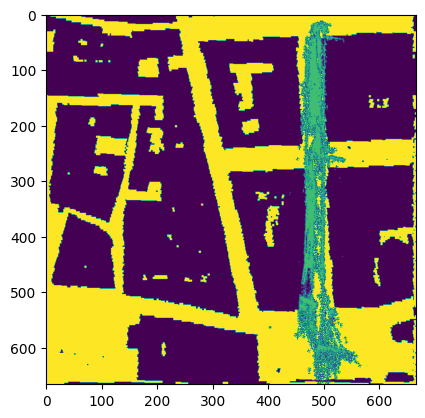
\includegraphics[width=\linewidth]{images/full/easy/5_6_2_easy}
            \caption{Easy: \textcolor{teal}{Success}}
            \label{fig:5_6_2_easy}
        \end{subfigure}
        \hfill
        \begin{subfigure}{0.45\textwidth}
            \centering
            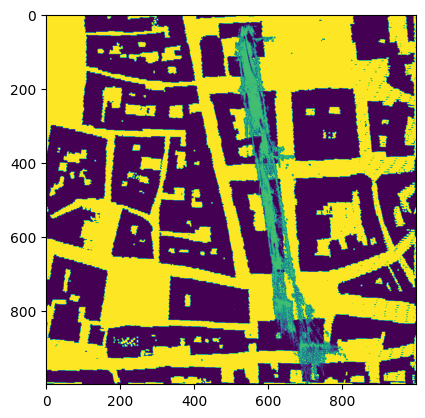
\includegraphics[width=\linewidth]{images/full/medium/5_6_2_medium}
            \caption{Medium: \textcolor{teal}{Success}}
            \label{fig:5_6_2_medium}
        \end{subfigure}

        \vspace{1em}

        \begin{subfigure}{0.45\textwidth}
            \centering
            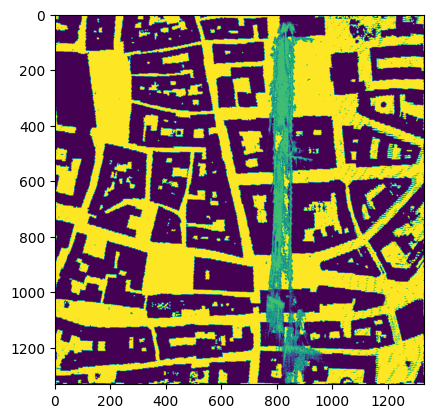
\includegraphics[width=\linewidth]{images/full/hard/5_6_2_hard}
            \caption{Hard: \textcolor{teal}{Success}}
            \label{fig:5_6_2_hard}
        \end{subfigure}
        \hfill

        \caption{Dataset 5}
        \label{fig:res_5_6_2}
    \end{figure}

    \begin{table}[p]
        \centering
        \begin{tabular}{|c|c|c|c|}
          \hline
          \textbf{Errors:} & \textbf{Transformation} & \textbf{Scale} & \textbf{Rotation} \\
          \hline
          \textbf{Easy}   & <1m  & -9.1\% & -3° \\
          \hline
          \textbf{Medium} & #TODO  & +27.2\% & +7° \\
          \hline
          \textbf{Hard}   & #TODO  & +81.2\% & -3° \\
          \hline
        \end{tabular}
        \caption{Detailed errors of Dataset 5}
        \label{tab:simpletable}
    \end{table}

    % 5_7_1
    \newpage
    \begin{figure}[p]
        \centering
        \begin{subfigure}{0.45\textwidth}
            \centering
            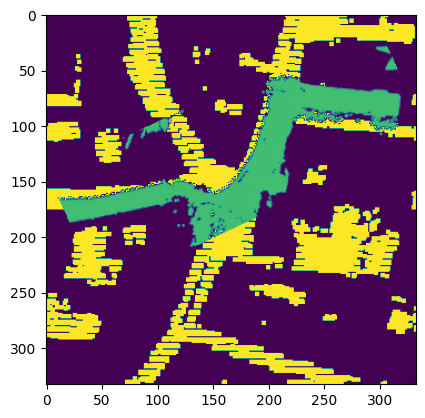
\includegraphics[width=\linewidth]{images/full/easy/5_7_1_easy}
            \caption{Easy: \textcolor{teal}{Success}}
            \label{fig:5_7_1_easy}
        \end{subfigure}
        \hfill
        \begin{subfigure}{0.45\textwidth}
            \centering
            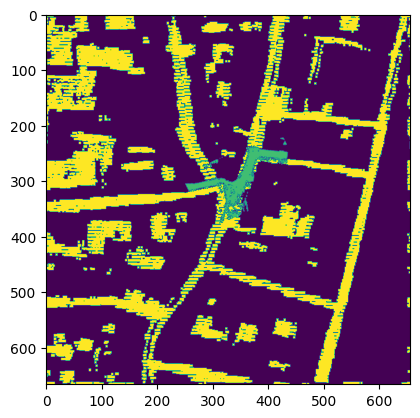
\includegraphics[width=\linewidth]{images/full/medium/5_7_1_medium}
            \caption{Medium: \textcolor{teal}{Success}}
            \label{fig:5_7_1_medium}
        \end{subfigure}

        \vspace{1em}

        \begin{subfigure}{0.45\textwidth}
            \centering
            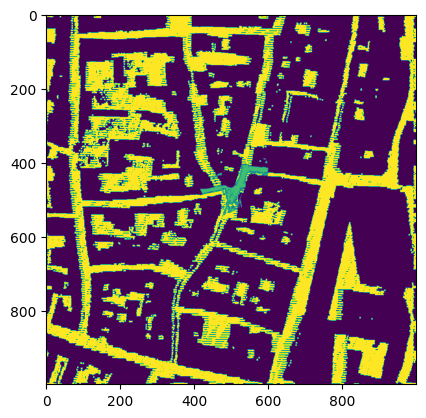
\includegraphics[width=\linewidth]{images/full/hard/5_7_1_hard}
            \caption{Hard: \textcolor{teal}{Success}}
            \label{fig:5_7_1_hard}
        \end{subfigure}
        \hfill

        \caption{Dataset 6}
        \label{fig:res_5_7_1}
    \end{figure}

    \begin{table}[p]
        \centering
        \begin{tabular}{|c|c|c|c|}
          \hline
          \textbf{Errors:} & \textbf{Transformation} & \textbf{Scale} & \textbf{Rotation} \\
          \hline
          \textbf{Easy}   & 1.4m  & +6.1\% & +3° \\
          \hline
          \textbf{Medium} & 3.6m  & +3.3\% & +3° \\
          \hline
          \textbf{Hard}   & 3.5m  & +3.3\% & +3° \\
          \hline
        \end{tabular}
        \caption{Detailed errors of Dataset 6}
        \label{tab:simpletable}
    \end{table}

    % 5_2_4
    \newpage
    \begin{figure}[p]
        \centering
        \begin{subfigure}{0.45\textwidth}
            \centering
            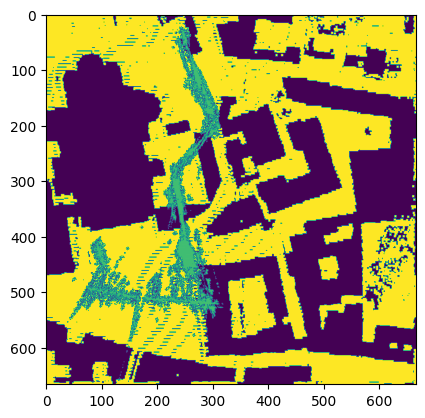
\includegraphics[width=\linewidth]{images/full/easy/5_2_4_easy}
            \caption{Easy: \textcolor{teal}{Success}}
            \label{fig:5_2_4_easy}
        \end{subfigure}
        \hfill
        \begin{subfigure}{0.45\textwidth}
            \centering
            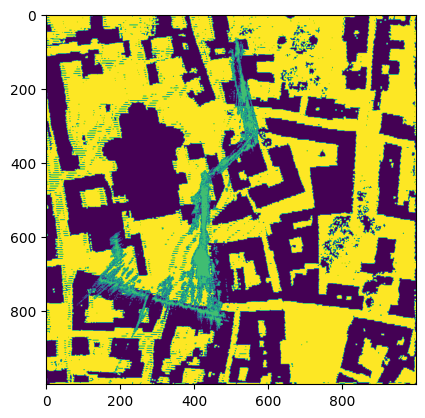
\includegraphics[width=\linewidth]{images/full/medium/5_2_4_medium}
            \caption{Medium: \textcolor{red}{Failed}}
            \label{fig:5_2_4_medium}
        \end{subfigure}

        \vspace{1em}

        \begin{subfigure}{0.45\textwidth}
            \centering
            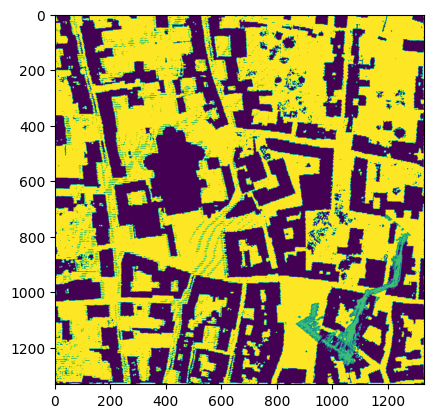
\includegraphics[width=\linewidth]{images/full/hard/5_2_4_hard}
            \caption{Hard: \textcolor{red}{Failed}}
            \label{fig:5_2_4_hard}
        \end{subfigure}
        \hfill

        \caption{Dataset 7}
        \label{fig:res_5_2_4}
    \end{figure}

    \begin{table}[p]
        \centering
        \begin{tabular}{|c|c|c|c|}
          \hline
          \textbf{Errors:} & \textbf{Transformation} & \textbf{Scale} & \textbf{Rotation} \\
          \hline
          \textbf{Easy}   & 34m  & -5.9\% & +4° \\
          \hline
          \textbf{Medium} & -  & - & - \\
          \hline
          \textbf{Hard}   & -  & - & - \\
          \hline
        \end{tabular}
        \caption{Detailed errors of Dataset 7}
        \label{tab:simpletable}
    \end{table}

    % 5_7_2
    \newpage
    \begin{figure}[p]
        \centering
        \begin{subfigure}{0.45\textwidth}
            \centering
            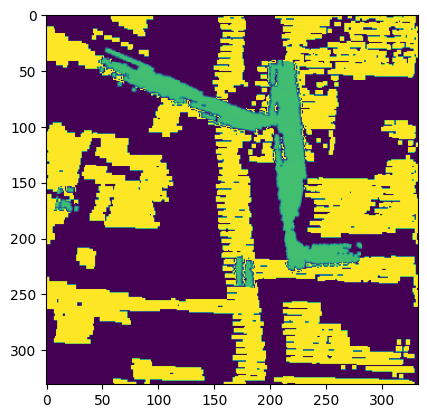
\includegraphics[width=\linewidth]{images/full/easy/5_7_2_easy}
            \caption{Easy: \textcolor{teal}{Success}}
            \label{fig:5_7_2_easy}
        \end{subfigure}
        \hfill
        \begin{subfigure}{0.45\textwidth}
            \centering
            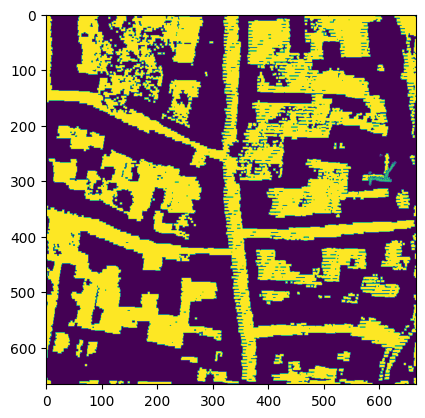
\includegraphics[width=\linewidth]{images/full/medium/5_7_2_medium}
            \caption{Medium: \textcolor{red}{Failed}}
            \label{fig:5_7_2_medium}
        \end{subfigure}

        \vspace{1em}

        \begin{subfigure}{0.45\textwidth}
            \centering
            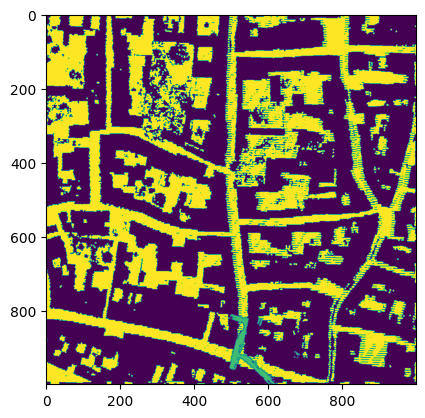
\includegraphics[width=\linewidth]{images/full/hard/5_7_2_hard}
            \caption{Hard: \textcolor{red}{Failed}}
            \label{fig:5_7_2_hard}
        \end{subfigure}
        \hfill

        \caption{Dataset 8}
        \label{fig:res_5_7_2}
    \end{figure}

    \begin{table}[p]
        \centering
        \begin{tabular}{|c|c|c|c|}
          \hline
          \textbf{Errors:} & \textbf{Transformation} & \textbf{Scale} & \textbf{Rotation} \\
          \hline
          \textbf{Easy}   & 17.2m  & -5.2\% & +1° \\
          \hline
          \textbf{Medium} & -  & - & - \\
          \hline
          \textbf{Hard}   & -  & - & - \\
          \hline
        \end{tabular}
        \caption{Detailed errors of Dataset 8}
        \label{tab:simpletable}
    \end{table}

    % 5_6_1
    \newpage
    \begin{figure}[p]
        \centering
        \begin{subfigure}{0.45\textwidth}
            \centering
            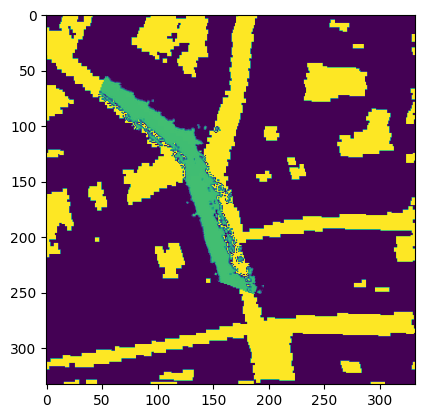
\includegraphics[width=\linewidth]{images/full/easy/5_6_1_easy}
            \caption{Easy: \textcolor{teal}{Success}}
            \label{fig:5_6_1_easy}
        \end{subfigure}
        \hfill
        \begin{subfigure}{0.45\textwidth}
            \centering
            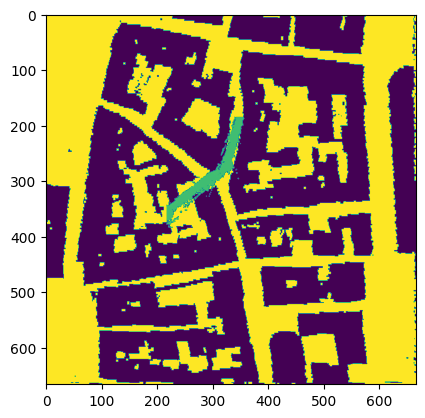
\includegraphics[width=\linewidth]{images/full/medium/5_6_1_medium}
            \caption{Medium: \textcolor{red}{Failed}}
            \label{fig:5_6_1_medium}
        \end{subfigure}

        \vspace{1em}

        \begin{subfigure}{0.45\textwidth}
            \centering
            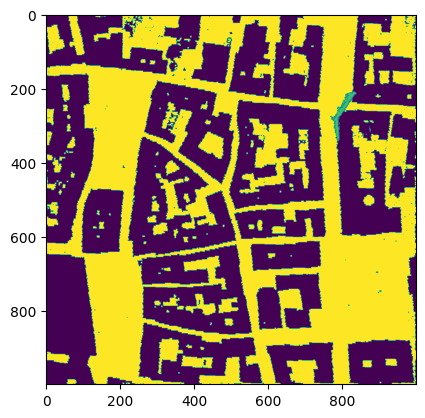
\includegraphics[width=\linewidth]{images/full/hard/5_6_1_hard}
            \caption{Hard: \textcolor{red}{Failed}}
            \label{fig:5_6_1_hard}
        \end{subfigure}
        \hfill

        \caption{Dataset 9}
        \label{fig:res_5_7_2}
    \end{figure}

    \begin{table}[p]
        \centering
        \begin{tabular}{|c|c|c|c|}
          \hline
          \textbf{Errors:} & \textbf{Transformation} & \textbf{Scale} & \textbf{Rotation} \\
          \hline
          \textbf{Easy}   & <1m  & -1.33\% & -3° \\
          \hline
          \textbf{Medium} & -  & - & - \\
          \hline
          \textbf{Hard}   & -  & - & - \\
          \hline
        \end{tabular}
        \caption{Detailed errors of Dataset 9}
        \label{tab:simpletable}
    \end{table}


    % 5_2_3
    \newpage
    \begin{figure}[p]
        \centering
        \begin{subfigure}{0.45\textwidth}
            \centering
            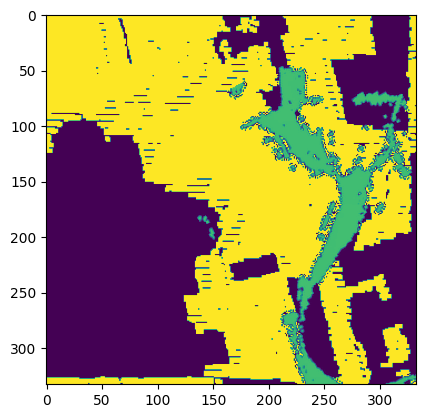
\includegraphics[width=\linewidth]{images/full/easy/5_2_3_easy}
            \caption{Easy: \textcolor{red}{Failed}}
            \label{fig:5_2_3_easy}
        \end{subfigure}
        \hfill
        \begin{subfigure}{0.45\textwidth}
            \centering
            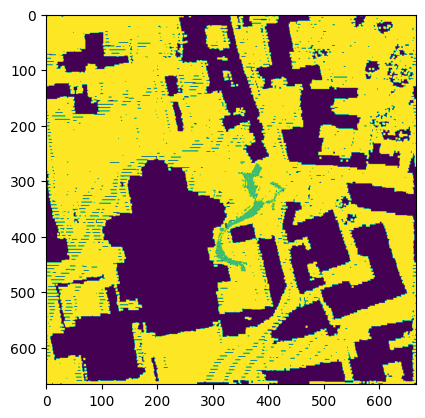
\includegraphics[width=\linewidth]{images/full/medium/5_2_3_medium}
            \caption{Medium: \textcolor{red}{Failed}}
            \label{fig:5_2_4_medium}
        \end{subfigure}

        \vspace{1em}

        \begin{subfigure}{0.45\textwidth}
            \centering
            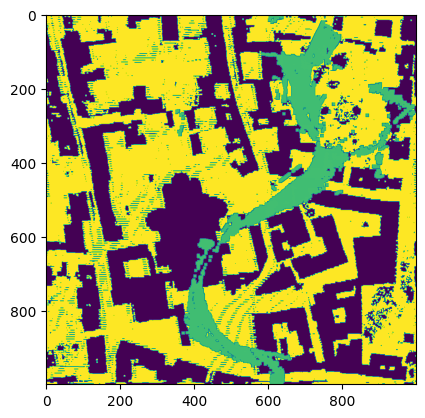
\includegraphics[width=\linewidth]{images/full/hard/5_2_3_hard}
            \caption{Hard: \textcolor{red}{Failed}}
            \label{fig:5_2_3_hard}
        \end{subfigure}
        \hfill

        \caption{Dataset 10}
        \label{fig:res_5_2_3}
    \end{figure}


\end{document}